\documentclass[12pt,twoside]{article}
\usepackage[dvipsnames]{xcolor}
\usepackage{tikz,graphicx,amsmath,amsfonts,amscd,amssymb,bm,cite,epsfig,epsf,url}
\usepackage[hang,flushmargin]{footmisc}
\usepackage[colorlinks=true,urlcolor=blue,citecolor=blue]{hyperref}
\usepackage{amsthm,multirow,wasysym,appendix}
\usepackage{array,subcaption} 
% \usepackage[small,bf]{caption}
\usepackage{bbm}
\usepackage{pgfplots}
\usetikzlibrary{spy}
\usepgfplotslibrary{external}
\usepackage{graphicx}
\usepgfplotslibrary{fillbetween}
\usetikzlibrary{arrows,automata}
\usepackage{thmtools}
\usepackage{blkarray} 
\usepackage{textcomp}
\usepackage{pgf,tikz}
\newcommand{\red}[1]{{\leavevmode\color{red}{#1}}}
\newcommand{\blue}[1]{{\leavevmode\color{blue}{#1}}}
\usepackage{pgfplots}
\usepackage[left=0.8in,right=1.0in,top=1.0in,bottom=1.0in]{geometry}

\input{macros}

\begin{document}

\begin{center}
{\large{\textbf{Homework 0}} } \vspace{0.2cm}\\
Due September 11 at 11 pm
\\
\end{center}


This homework will help you review key mathematical concepts that we
will need in the course.
\begin{enumerate}

\item (Sets) We will use set theory to define probability spaces. Are these statements true or false? Provide a proof if they are true (you can use Venn diagrams to gain intuition, but also write down a formal proof), or a counterexample if they are false. 
\begin{enumerate}
\item[] A partition of a set $\Omega$ is a collection of sets $S_1$, \ldots, $S_n$ such that $\Omega = \cup_{i}S_i$ and $S_i \cap S_j = \emptyset$ for $i\neq j$. 
\item If  $S_1$, \ldots, $S_n$ is a partition of $\Omega$, then for any subset $A \subseteq \Omega$, $S_1 \cap A$, \ldots, $S_n \cap A$ is a partition of $A$.
\blue{
\begin{enumerate}
    \item to show $S_1\cap A \cup ..... \cup S_n\cap A$ is a partition of A we first want to show $U_{i=1}^{n}S_i\cap A=A$
    \begin{itemize}
        \item so consider $(S_1\cap A)\cup(S_2\cap A)\cup....\cup(S_N\cap A)$ we know by de morgans law we can re-write this as
        $((S_1\cup S_2)\cap A)cup (S_3\cap A)\cup...(S_n\cap A)$ this can be repeated until we have $(\Cup_{i=1}^{n}S_i)\cap A$ since we know $S_1..S_n$ is a partition of the sample space we can write  $(\Cup_{i=1}^{n}S_i)\cap A= \Omega\cap A$ where A is a subset of the sample space thus $(\Cup_{i=1}^{n}S_i)\cap A= \Omega\cap A=A$
    \end{itemize}
    \item next we would like to show that $(S_i\cap A)\cap (S_j \cap A)= \emptyset$
    \begin{itemize}
        \item consider an arbitrary $i,j\in [0,n]$ such that $i\neq j$ this gives us $(S_i\cap A)\cap (S_j \cap A)$ but we know that intersection is cumulative so thus we have $(S_i\cap S_j)\cap (A)$ and given $i\neq j$ we have $(S_i\cap S_j)=\emptyset$ thus we have  $(S_i\cap A)\cap (S_j \cap A)=(S_i\cap S_j)\cap (A)=\emptyset \cap A = \emptyset$ 
    \end{itemize}
\end{enumerate}
}



\item For any sets $A$ and $B$, $A^c \cup B^c = (A \cup B)^c$. 
\blue{
\begin{itemize}
    \item the statement is false as a counter example consider $\Omega=\{0,1\} A=\{0\}, B=\{1\}$
    \item $A^c\cup B^c=\{1\}\cup\{0\}=\{0,1\}\neq (A\cup B)^c=\emptyset$
\end{itemize}
}

\item For any sets $A$, $B$, and $C$, $(A \cup B) \cap C = A \cup (B \cap C)$. 
\blue{
\begin{itemize}
    \item this is false 
    \item consider $A=\{0\}, B=\{1\}, C=\{2\}$
    \item $(A\cup B)\cap C=\{0,1\}\cap\{2\}=\emptyset \neq A\cap(B\cup C)=\{0\}\cap\emptyset=\{0\}$
\end{itemize}


}


\end{enumerate}
% \vspace{0.4cm}

\item (Series) We will need series to compute probabilities and expectations related to discrete quantities. 
 \begin{enumerate}
\item  Assuming $r\neq 1$, derive a simple expression for
\begin{align}
S_n := \sum_{i=m}^{n} r^{i}
\end{align}
as a function of $r$, $m$ and $n$, and prove that it holds. Assume $m$
and $n$ are positive integers with $m\leq n$.


\blue{

\begin{itemize}
    \item given $S_n = \sum_{i=m}^{n} r^{i}=r^m+r^{m+1}+...+r^n$ we can multiply $S_n$ by r to shift the index one over $r*S_n = \sum_{i=m+1}^{n+1} r^{i}=r^{m+1}+r^{m+2}+...+r^{n+1}$ then if we subtract the $S_n-r*S_n$ we get $S_n-r*S_n=r^m+r^{m+1}+...+r^n-r^{m+1}+r^{m+2}+...+r^{n+1}$ which simplfies to $(1-r)S_n=r_m-r_{n+1}$ finally yielding $S_n=\frac{r_m-r_{n+1}}{1-r}$ 
\end{itemize}

}



\item Under what condition on $r$ does the infinite series
\begin{align}
\sum_{i=m}^{\infty} r^{i} = \lim_{n \rightarrow \infty} S_n
\end{align}
converge (where again $m$ is a positive integer)?  
\blue{
\\ three cases must be considered 
\begin{enumerate}
    \item first $r\geq1$
    \begin{itemize}
        \item in this case it is plane to see that $\sum_{i=m}^{\infty} r^{i} = \lim_{n \rightarrow \infty} S_n$ can not converge by looking at $\lim_{n \rightarrow \infty}\sum_{i=m}^{n} r^{i} =r^m+...+r^n$ so the final term will be $\lim_{n \rightarrow \infty}r^n$ but as $r\geq 1$ this quantity will continue to grow that is $\lim_{n \rightarrow \infty}r^n\neq 0$ and thus under this condition the series will not converge
    \end{itemize}
    \item second consider $r\in(-1,1)$
    \begin{itemize}
    \item  looking at the series of partial sums yields $\lim_{n \rightarrow \infty}\sum_{i=m}^{n} r^{i} =r^m+...+r^n$ that is the final term will be $\lim_{n \rightarrow \infty}r^n=\lim_{n \rightarrow \infty}\Pi_{i=m}^{n}=r*r*(\lim_{n \rightarrow \infty}\Pi_{i=m+2}^{n})$ as $r\in(-1,1)$ we see that $r*r\leq r$ this can continue for all values and at the limit we will have $\lim_{n \rightarrow \infty}r^n=\lim_{n \rightarrow \infty}\Pi_{i=m}^{n}=0$ thus under this condition the series will converge 
    \end{itemize}
    \item finally consider $r\leq-1$
        \begin{itemize}
      \item in this case it is plane to see that $\sum_{i=m}^{\infty} r^{i} = \lim_{n \rightarrow \infty} S_n$ can not converge by looking at $\lim_{n \rightarrow \infty}\sum_{i=m}^{n} r^{i} =r^m+...+r^n$ so the final term will be $\lim_{n \rightarrow \infty}r^n$ but as $r\leq -1$ this quantity will continue in terms of absolute value and thus $\lim_{n \rightarrow \infty}r^n\neq 0$ and thus under this condition the series will not converge 
    \end{itemize}
\end{enumerate}
\\ so in closing the series will only converge when $r\in(-1,1)$}


\item Use induction to prove the identity
\begin{align}
\sum_{i=1}^{n} i = \frac{n(n+1)}{2},
\end{align}
where $n$ is a nonnegative integer greater than 1.
\end{enumerate}

\blue{
\begin{itemize}
    \item let us first check the base case $i=2$ so that would be $\Sigma_{i=1}^{2}i=1+2=3=\frac{6}{2}=\frac{2(2+1)}{2}$ so yeah the base case holds
    \item for our induction hypothesis step we assume that this property holds for all integers $k\in [2,n]$
    \item then for our inductive step we want to show this proerty holds for $n+1$. so we know $\Sigma_{i=1}^{n+1}i=(n+1)+\Sigma_{i=1}^{n}i=(n+1)+\frac{n(n+1)}{2}=\frac{2(n+1)+n(n+1)}{2}=\frac{(2+n)(n+1)}{2}$ which is what we wanted to show
\end{itemize}

}

\item (Derivatives) We will use derivatives to define probability density functions. The derivative of a differentiable function $f$ is defined as 
\begin{align}
f'(x) := \lim_{h \rightarrow 0} \frac{f(x+h) - f(x)}{h}.
\end{align}
  \begin{enumerate}
  \item Briefly explain why the derivative of a function can be interpreted as an \emph{instantaneous rate of change}.
  \blue{
  \begin{itemize}
      \item breaking the question into parts, put simply the rate of change of a function is the slope that is $ \frac{f(x+h) - f(x)}{h}$ as we bring this h to its limit that is take the rate of change at an infinitesimal distance we get $\lim_{h \rightarrow 0} \frac{f(x+h) - f(x)}{h}$ that is the rate of change at that instant ie the instantaneous rate of change
      \item I think physics helps, just keep in mind that the derivative of movement is velocity. 
  \end{itemize}
  }
  
  \item Use the definition to derive the derivative of the function $x^2$.
  \blue{
  \begin{itemize}
  \item $f'(x)= \lim_{h \rightarrow 0} \frac{f(x+h) - f(x)}{h}=\lim_{h \rightarrow 0} \frac{(x+h)^2 - (x)^2}{h}$
  \item $\lim_{h \rightarrow 0}\frac{x^2+2xh+h^2 - x^2}{h}=\lim_{h \rightarrow 0} \frac{2xh+h^2}{h}=\lim_{h \rightarrow 0} 2x+h=2x$
  \end{itemize}
  }
  
  
  \item We would like to approximate a differentiable function $f$ at
    $y$ using a linear function $L_y(x):=ax + b$. We set $a$ and $b$
    so that $f$ and $L_y$ have the same value and the same derivative
    at $y$ (i.e., $L_y(y)=f(y)$ and $L_y'(y)=f'(y)$). Give an
    expression for $L_{y}(x)$ in terms of $y$, $f(y)$, and $f'(y)$.  
\blue{
\begin{itemize}
    \item the proper equation is $L_y(x)=f'(y)(x-y)+f(y)$
    \item we can verify this by checking our two conditions 
    \begin{itemize}
        \item $L_y(y)=f'(y)(y-y)+f(y)=0+f(y)=f(y)$
        \item $L_y'(y)=f''(y)(y-y)+f'(y)=f'(y)$
    \end{itemize}
    \item so our conditions are met. 
\end{itemize}

}    
    
    
  \item Let $f(x) = 4x^2 e^{x}$. Plot $f$ and $L_{2}$ between 1 and 3. 
    \blue{
    \begin{itemize}

  \item first of all we have $f'(x)=8xe^x+4x^2e^x$ so we get $L_2(x)=f'(2)(x-2)+f(2)=(8*2*e^{2}+4*2^2*e^{2})(x-2)+4*2^2*e^{2}$ 
  \item the scaling is a bit weird so i just labeled my graph the best i could
\\\includegraphics[width=15cm]{homework 0/img.jpg}
    \end{itemize}
 
  }
  \end{enumerate}
 \item (Integrals) We will use integrals to compute probabilities and expectations related to continuous quantities.
 \begin{enumerate}
 \item Express the area of the following shape in terms of an integral
   and solve it. Each of the four bounding curves are graphs of
   quadratic functions.  As depicted, the bounding curve includes the
   points $(0,1)$, $(1,0)$, and $(1/2,1/4)$, and is symmetric about
   the $x$ and $y$ axes.
 \begin{center}
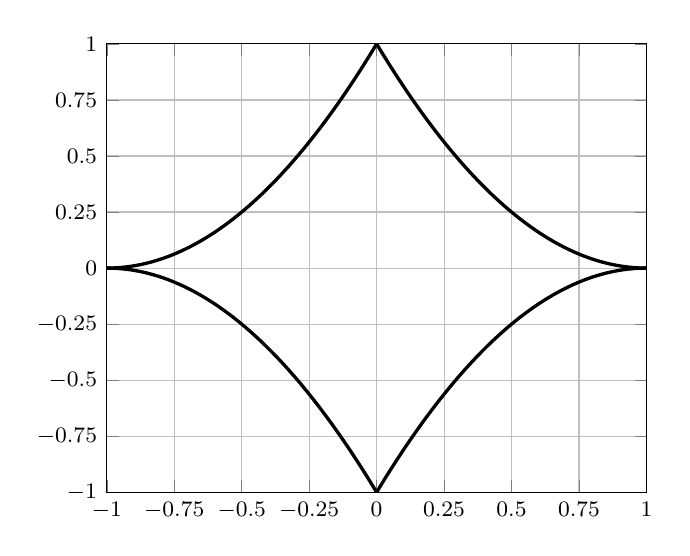
\begin{tikzpicture}
\begin{axis}[grid=major, xtick={-1,-0.75,...,1}, ytick={-1,-0.75,...,1}, xmin= -1, xmax=1, ymin=-1, ymax=1,tick label style={font=\footnotesize}]
\addplot[ very thick,samples=500] {(x-1)^2} ;
\addplot[ very thick,samples=500] {(-x-1)^2} ;
\addplot[ very thick,samples=500] {-(x-1)^2} ;
\addplot[ very thick,samples=500] {-(-x-1)^2} ;
\end{axis}
\end{tikzpicture}
\end{center}
\blue{
\begin{itemize}
    \item i was not sure if you wanted us to consider negative area or not. 
    \item if we consider area bellow y=0 negative the area is 
    \begin{itemize}
    \item we can express this area as the sum of 4 integrals.
    \item quadrant one can be written $\int_{0}^{1}(1-x)^2dx=\frac{1}{3}(1-x)^3|_{0}^{1}=\frac{1}{3}$ 
    \item quadrant two can be written as $\int_{-1}^{0}(-x-1)^2dx=\frac{-1}{3}(-x-1)^3|_{-1}^{0}=\frac{1}{3}$
    \item quadrant three can be written as $\int_{-1}^{0}-(-x-1)^2dx=-\int_{-1}^{0}(-x-1)^2dx=-\frac{-1}{3}(-x-1)^3|_{-1}^{0}=-\frac{1}{3}$
    \item quadrant four can be written $\int_{0}^{1}-(1-x)^2dx=-\int_{0}^{1}(1-x)^2dx=-\frac{1}{3}(1-x)^3|_{0}^{1}=-\frac{1}{3}$ 
    \item finally this gives us a total area of $\frac{1}{3}+\frac{1}{3}-\frac{1}{3}-\frac{1}{3}=0$
    \end{itemize}
    \item if we consider all area positive we can do it slightly differently. 
    \begin{itemize}
        \item quadrant one can be written $\int_{0}^{1}(1-x)^2dx=\frac{1}{3}(1-x)^3|_{0}^{1}=\frac{1}{3}$ 
        \itme since we know that the shape is symmetric, we can multiply this by 4 to get the total area. so the total area is $4*\int_{0}^{1}(1-x)^2dx=\frac{4}{3}$
    \end{itemize}
\end{itemize}

}
  \item Use change of variables to derive a closed-form expression for the function
 \begin{align}
f(t) := \int_{0}^{t} \frac{x}{1+x^2} \diff{x}.
 \end{align}
\blue{
\begin{itemize}
    \item starting with $\int_{0}^{t} \frac{x}{1+x^2} \diff{x}$ we cab gave $u=1+x^2, du=2xdx$ which can be re-writen as $\frac{1}{2}du=xdx$ 
    \item we know need to change our bounds to $[1,1+t^2]$ 
    \item finally we can rewrite teh integral as  $f(t)=\frac{1}{2}\int_{1}^{1+t^2} \frac{1}{u} \diff{u}=\frac{1}{2}(ln|u|)|_{1}^{1+t^2}=\frac{1}{2}(ln|1+t^2|-ln|1|)=\frac{1}{2}(ln|1+t^2|)$
\end{itemize}
}
\end{enumerate}

%\item (Gradients)
%Recall that the entries of the gradient of a function are equal to its partial derivatives. Use this fact to: 
%\begin{enumerate}
%\item Compute the gradient of $f(x) = b^T x$ where $b \in \R^{d}$ and $f: \R^{d} \rightarrow \R $.
%\item Compute the gradient of $f(x) = x^T A x$ where $A \in \R^{d\times d}$ and $f: \R^{d} \rightarrow \R $.
%\end{enumerate}
  
\end{enumerate}
\end{document}
